\chapter{Results}

\section{Overview}

This chapter presents the measured results in three parts.
Section~\ref{sec:harness-val} reports the harness validation, which establishes
that the timing infrastructure is trustworthy.
Section~\ref{sec:exec-time} reports the execution-time results across message
sizes and optimization levels.
Section~\ref{sec:throughput} reports the throughput results in cycles per byte.
Section~\ref{sec:code-size} reports the code-size results.
All timing figures are cycle counts at 48\,MHz, where one timer tick equals one
processor cycle.
All results derive from the single consolidated data set, and every figure and
table is reproducible from it.

\section{Harness Validation}
\label{sec:harness-val}

The \texttt{memcpy} validation passed all four checks on both boards.
The measured time grew in proportion to the input size, the per-iteration
variation was zero after the discarded warmup run, the smallest input size
recorded a non-zero time, and both boards reported the expected 48\,MHz clock.
The per-iteration determinism observed here persisted through all later
measurements: across the cryptographic benchmarks the median, minimum, and
maximum coincided for every measured point, so the timing results are reported
as single median values without dispersion.

The ratio between the two boards for the \texttt{memcpy} workload settled at
approximately 2.8 to~1 at the largest size, with the Cortex-M0 slower than the
Cortex-M4F at the same clock.
This figure is the architectural baseline against which the cryptographic ratios
in the following sections are read.

\section{Execution Time}
\label{sec:exec-time}

\subsection{Runtime Across Message Sizes}

Figure~\ref{fig:runtime} shows median execution time against input size on
logarithmic axes, with one panel per board, at optimization level \texttt{-O2}.
On both boards Ascon-AEAD128 is faster than AES-128-GCM at every measured size.
The curves share a characteristic shape: at the smallest sizes the time is
nearly constant, because the fixed per-call cost dominates; above approximately
100 bytes the time rises in proportion to the input size, which is the per-byte
encryption cost.
The vertical separation between the two algorithms is present across the whole
range and is wider on the Cortex-M0 board than on the Cortex-M4F board.

\begin{figure}[htbp]
  \centering
  
\includegraphics[width=\linewidth]{runtime_vs_size_O2}
  \caption{Median execution time vs.\ message size at \texttt{-O2} on both
           boards (logarithmic axes). Ascon-AEAD128 is consistently faster than
           AES-128-GCM at every size.}
  \label{fig:runtime}
\end{figure}

\subsection{Effect of Optimization Level}

Figure~\ref{fig:optsweep} shows median execution time at a fixed message size of
1000 bytes across the five optimization levels, with one panel per board and a
logarithmic time axis.
Table~\ref{tbl:timing-1000} gives the underlying values.

\begin{figure}[htbp]
  \centering
  
\includegraphics[width=\linewidth]{opt_sweep_1000B}
  \caption{Median execution time at 1000\,bytes across optimization levels on
           both boards (logarithmic time axis).}
  \label{fig:optsweep}
\end{figure}

The dominant effect is the step from \texttt{-O0} to \texttt{-O1}.
On the Cortex-M0 the Ascon-AEAD128 time at 1000 bytes falls from 1{,}387{,}063
cycles at \texttt{-O0} to 170{,}741 cycles at \texttt{-O1}, a factor of about
eight.
The AES-128-GCM time falls from 2{,}661{,}457 to 792{,}911 cycles over the same
step, a factor of about three.
On the Cortex-M4F the same step takes Ascon-AEAD128 from 726{,}789 to 104{,}422
cycles and AES-128-GCM from 845{,}537 to 242{,}980 cycles.

Between \texttt{-O1}, \texttt{-O2}, and \texttt{-O3} the changes are smaller
and not uniform.
On the Cortex-M4F, AES-128-GCM is essentially unchanged from \texttt{-O2} to
\texttt{-O3} (193{,}311 and 193{,}283 cycles), while Ascon-AEAD128 improves
from 98{,}262 to 70{,}194 cycles.
On the Cortex-M0, AES-128-GCM improves notably at \texttt{-O3}, from 770{,}536
to 485{,}227 cycles, while Ascon-AEAD128 improves modestly, from 168{,}921 to
145{,}888 cycles.

At \texttt{-Os} both algorithms are slower than at \texttt{-O2} on both boards.
On the Cortex-M0 the Ascon-AEAD128 time at \texttt{-Os} is 268{,}899 cycles,
slower than its \texttt{-O1} time.
On the Cortex-M4F the corresponding \texttt{-Os} time is 139{,}993 cycles.

\begin{table}[htbp]
  \centering
  \caption{Median execution time (cycles) and ratio at 1000\,bytes per
           optimization level.}
  \label{tbl:timing-1000}
  \begin{tabular}{lrrrrrr}
    \toprule
    Level &
    \multicolumn{1}{c}{M0 ASCON} &
    \multicolumn{1}{c}{M0 AES} &
    \multicolumn{1}{c}{M0 ratio} &
    \multicolumn{1}{c}{M4 ASCON} &
    \multicolumn{1}{c}{M4 AES} &
    \multicolumn{1}{c}{M4 ratio} \\
    \midrule
    \texttt{-O0} & 1{,}387{,}063 & 2{,}661{,}457 & 1.92 & 726{,}789 & 845{,}537 & 1.16 \\
    \texttt{-O1} &   170{,}741   &   792{,}911   & 4.64 & 104{,}422 & 242{,}980 & 2.33 \\
    \texttt{-O2} &   168{,}921   &   770{,}536   & 4.56 &  98{,}262 & 193{,}311 & 1.97 \\
    \texttt{-O3} &   145{,}888   &   485{,}227   & 3.33 &  70{,}194 & 193{,}283 & 2.75 \\
    \texttt{-Os} &   268{,}899   &   787{,}284   & 2.93 & 139{,}993 & 269{,}250 & 1.92 \\
    \bottomrule
  \end{tabular}
\end{table}

At \texttt{-O0} the two algorithms are close, especially on the Cortex-M4F
where the ratio is 1.16.
Once optimization is enabled the ratio is larger, and at every optimized level
the ratio is greater on the Cortex-M0 than on the Cortex-M4F.
The largest ratio in favor of Ascon-AEAD128 occurs at \texttt{-O1} and
\texttt{-O2} on the Cortex-M0, at approximately 4.6.

\section{Throughput}
\label{sec:throughput}

Figure~\ref{fig:cpb} shows median cycles per byte against input size on
logarithmic axes, with one panel per board, at \texttt{-O2}.
At the smallest size the cost per byte is highest, because the fixed per-call
cost is divided across a single byte.
As the message grows the cost per byte falls toward a flat asymptote, which is
the per-byte encryption rate.

\begin{figure}[htbp]
  \centering
  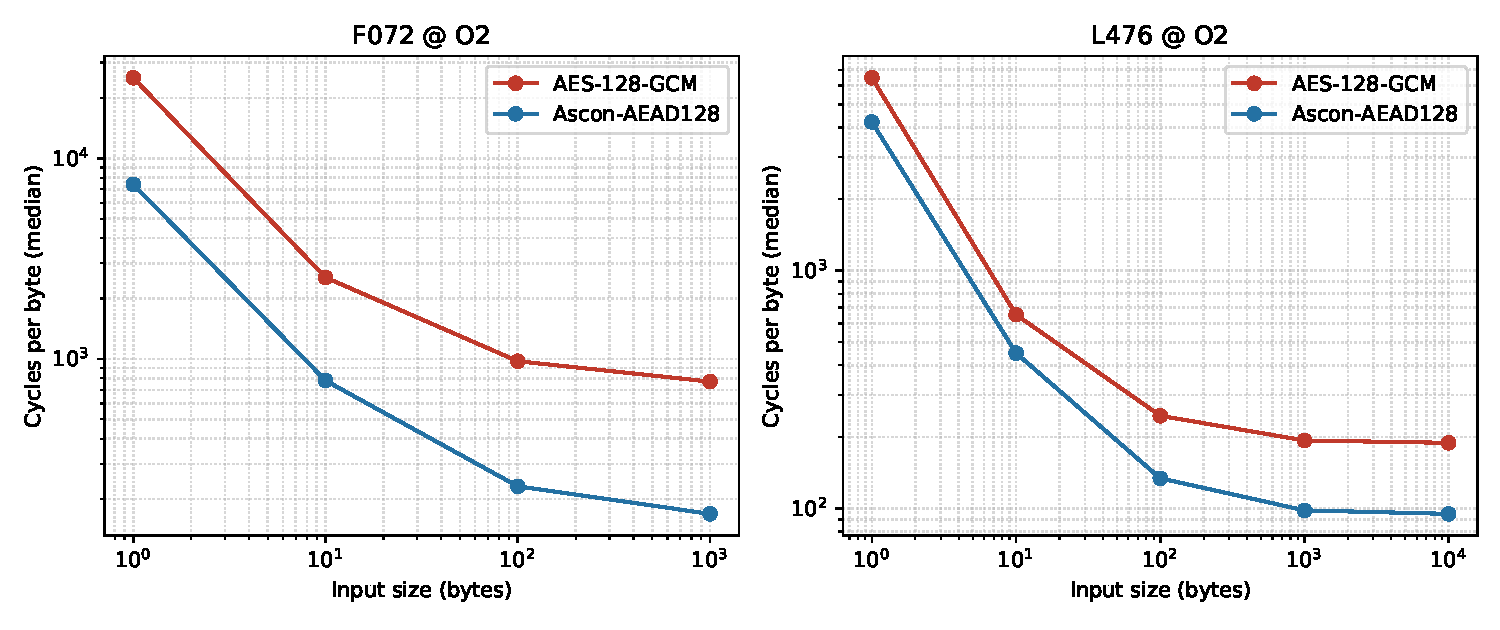
\includegraphics[width=\linewidth]{cycles_per_byte_O2}
  \caption{Median cycles per byte vs.\ message size at \texttt{-O2} on both
           boards (logarithmic axes). The asymptotic value at large sizes
           reflects the steady-state per-byte encryption rate.}
  \label{fig:cpb}
\end{figure}

In the large-message region the per-byte rates at \texttt{-O2} are as follows.
On the Cortex-M0 at 1000 bytes, Ascon-AEAD128 reaches approximately 169 cycles
per byte and AES-128-GCM approximately 771 cycles per byte.
On the Cortex-M4F at 10{,}000 bytes, Ascon-AEAD128 reaches approximately
95 cycles per byte and AES-128-GCM approximately 189 cycles per byte.

At the smallest message size of one byte, where the figure reflects the fixed
per-call cost, the values at \texttt{-O2} are 7{,}410 cycles for Ascon-AEAD128
and 25{,}185 cycles for AES-128-GCM on the Cortex-M0, and 4{,}219 cycles for
Ascon-AEAD128 and 6{,}470 cycles for AES-128-GCM on the Cortex-M4F.

\section{Code Size}
\label{sec:code-size}

Figure~\ref{fig:footprint} shows the marginal Flash cost of each algorithm at
\texttt{-Os} for both boards.
Table~\ref{tbl:footprint} gives the marginal Flash cost at every optimization
level.

\begin{figure}[htbp]
  \centering
  
\includegraphics[width=0.75\linewidth]{footprint_flash_Os}
  \caption{Marginal Flash cost at \texttt{-Os} for each algorithm and board.
           Ascon-AEAD128 requires approximately 3.8$\times$ less Flash than
           AES-128-GCM at this level.}
  \label{fig:footprint}
\end{figure}

At \texttt{-Os}, Ascon-AEAD128 adds 4{,}376 bytes of Flash on the Cortex-M0
and 4{,}208 bytes on the Cortex-M4F.
AES-128-GCM adds 16{,}500 bytes on the Cortex-M0 and 15{,}776 bytes on the
Cortex-M4F.
The ratio of AES-128-GCM to Ascon-AEAD128 marginal Flash is approximately 3.8
on both boards.

\begin{table}[htbp]
  \centering
  \caption{Marginal Flash cost (bytes) and ratio per optimization level.}
  \label{tbl:footprint}
  \begin{tabular}{lrrrrrr}
    \toprule
    Level &
    \multicolumn{1}{c}{M0 AES} &
    \multicolumn{1}{c}{M0 ASCON} &
    \multicolumn{1}{c}{M0 ratio} &
    \multicolumn{1}{c}{M4 AES} &
    \multicolumn{1}{c}{M4 ASCON} &
    \multicolumn{1}{c}{M4 ratio} \\
    \midrule
    \texttt{-O0} & 26{,}296 & 12{,}836 & 2.05 & 23{,}256 &  6{,}776 & 3.43 \\
    \texttt{-O1} & 17{,}396 & 27{,}924 & 0.62 & 16{,}496 & 24{,}208 & 0.68 \\
    \texttt{-O2} & 17{,}476 & 27{,}504 & 0.64 & 16{,}584 & 23{,}264 & 0.71 \\
    \texttt{-O3} & 24{,}208 & 43{,}024 & 0.56 & 17{,}720 & 34{,}560 & 0.51 \\
    \texttt{-Os} & 16{,}500 &  4{,}376 & 3.77 & 15{,}776 &  4{,}208 & 3.75 \\
    \bottomrule
  \end{tabular}
\end{table}

The Ascon-AEAD128 marginal Flash cost varies strongly with optimization level.
Figure~\ref{fig:footprint-levels} shows this for each board.
At \texttt{-Os} it is the smaller of the two algorithms by a wide margin.
At \texttt{-O1}, \texttt{-O2}, and \texttt{-O3} it is larger than the
AES-128-GCM cost, reaching a maximum at \texttt{-O3} of 43{,}024 bytes on the
Cortex-M0 and 34{,}560 bytes on the Cortex-M4F.
The AES-128-GCM marginal Flash cost is comparatively stable across levels,
between roughly 16{,}000 and 26{,}000 bytes.
The shape of the Ascon-AEAD128 curve is the same on both boards, rising from
\texttt{-O0} through a peak at \texttt{-O3} and then falling sharply at
\texttt{-Os}.

\begin{figure}[htbp]
  \centering
  
\includegraphics[width=0.49\linewidth]{footprint_across_levels_F072}%
  \hfill%
  
\includegraphics[width=0.49\linewidth]{footprint_across_levels_L476}
  \caption{Marginal Flash cost across all optimization levels. Left:
           Cortex-M0 (F072). Right: Cortex-M4F (L476). The Ascon-AEAD128
           cost varies strongly with optimization level due to permutation
           unrolling, while AES-128-GCM remains comparatively stable.}
  \label{fig:footprint-levels}
\end{figure}

\section{Summary of Results}

Across both boards and all message sizes, Ascon-AEAD128 executed faster than
AES-128-GCM at every optimization level.
The advantage was smallest at \texttt{-O0} and larger once optimization was
enabled.
At equal clock frequency the advantage was consistently larger on the Cortex-M0
than on the Cortex-M4F, reaching a factor of about 4.6 at 1000 bytes on the
Cortex-M0.
In code size, Ascon-AEAD128 was substantially smaller than AES-128-GCM at
\texttt{-Os}, by a factor of about 3.8 on both boards, while at the
speed-oriented optimization levels its reference implementation was larger than
AES-128-GCM due to the expansion of the permutation code.
These results are interpreted in relation to the four research questions in
Chapter~5.
